\documentclass[
  jou,
  floatsintext,
  longtable,
  nolmodern,
  notxfonts,
  notimes,
  colorlinks=true,linkcolor=blue,citecolor=blue,urlcolor=blue]{apa7}

\usepackage{amsmath}
\usepackage{amssymb}



\usepackage[bidi=default]{babel}
\babelprovide[main,import]{english}


% get rid of language-specific shorthands (see #6817):
\let\LanguageShortHands\languageshorthands
\def\languageshorthands#1{}

\RequirePackage{longtable}
\RequirePackage{threeparttablex}

\makeatletter
\renewcommand{\paragraph}{\@startsection{paragraph}{4}{\parindent}%
	{0\baselineskip \@plus 0.2ex \@minus 0.2ex}%
	{-.5em}%
	{\normalfont\normalsize\bfseries\typesectitle}}

\renewcommand{\subparagraph}[1]{\@startsection{subparagraph}{5}{0.5em}%
	{0\baselineskip \@plus 0.2ex \@minus 0.2ex}%
	{-\z@\relax}%
	{\normalfont\normalsize\bfseries\itshape\hspace{\parindent}{#1}\textit{\addperi}}{\relax}}
\makeatother




\usepackage{longtable, booktabs, multirow, multicol, colortbl, hhline, caption, array, float, xpatch}
\usepackage{subcaption}
\renewcommand\thesubfigure{\Alph{subfigure}}
\setcounter{topnumber}{2}
\setcounter{bottomnumber}{2}
\setcounter{totalnumber}{4}
\renewcommand{\topfraction}{0.85}
\renewcommand{\bottomfraction}{0.85}
\renewcommand{\textfraction}{0.15}
\renewcommand{\floatpagefraction}{0.7}

\usepackage{tcolorbox}
\tcbuselibrary{listings,theorems, breakable, skins}
\usepackage{fontawesome5}

\definecolor{quarto-callout-color}{HTML}{909090}
\definecolor{quarto-callout-note-color}{HTML}{0758E5}
\definecolor{quarto-callout-important-color}{HTML}{CC1914}
\definecolor{quarto-callout-warning-color}{HTML}{EB9113}
\definecolor{quarto-callout-tip-color}{HTML}{00A047}
\definecolor{quarto-callout-caution-color}{HTML}{FC5300}
\definecolor{quarto-callout-color-frame}{HTML}{ACACAC}
\definecolor{quarto-callout-note-color-frame}{HTML}{4582EC}
\definecolor{quarto-callout-important-color-frame}{HTML}{D9534F}
\definecolor{quarto-callout-warning-color-frame}{HTML}{F0AD4E}
\definecolor{quarto-callout-tip-color-frame}{HTML}{02B875}
\definecolor{quarto-callout-caution-color-frame}{HTML}{FD7E14}

%\newlength\Oldarrayrulewidth
%\newlength\Oldtabcolsep


\usepackage{hyperref}




\providecommand{\tightlist}{%
  \setlength{\itemsep}{0pt}\setlength{\parskip}{0pt}}
\usepackage{longtable,booktabs,array}
\usepackage{calc} % for calculating minipage widths
% Correct order of tables after \paragraph or \subparagraph
\usepackage{etoolbox}
\makeatletter
\patchcmd\longtable{\par}{\if@noskipsec\mbox{}\fi\par}{}{}
\makeatother
% Allow footnotes in longtable head/foot
\IfFileExists{footnotehyper.sty}{\usepackage{footnotehyper}}{\usepackage{footnote}}
\makesavenoteenv{longtable}

\usepackage{graphicx}
\makeatletter
\newsavebox\pandoc@box
\newcommand*\pandocbounded[1]{% scales image to fit in text height/width
  \sbox\pandoc@box{#1}%
  \Gscale@div\@tempa{\textheight}{\dimexpr\ht\pandoc@box+\dp\pandoc@box\relax}%
  \Gscale@div\@tempb{\linewidth}{\wd\pandoc@box}%
  \ifdim\@tempb\p@<\@tempa\p@\let\@tempa\@tempb\fi% select the smaller of both
  \ifdim\@tempa\p@<\p@\scalebox{\@tempa}{\usebox\pandoc@box}%
  \else\usebox{\pandoc@box}%
  \fi%
}
% Set default figure placement to htbp
\def\fps@figure{htbp}
\makeatother


% definitions for citeproc citations
\NewDocumentCommand\citeproctext{}{}
\NewDocumentCommand\citeproc{mm}{%
  \begingroup\def\citeproctext{#2}\cite{#1}\endgroup}
\makeatletter
 % allow citations to break across lines
 \let\@cite@ofmt\@firstofone
 % avoid brackets around text for \cite:
 \def\@biblabel#1{}
 \def\@cite#1#2{{#1\if@tempswa , #2\fi}}
\makeatother
\newlength{\cslhangindent}
\setlength{\cslhangindent}{1.5em}
\newlength{\csllabelwidth}
\setlength{\csllabelwidth}{3em}
\newenvironment{CSLReferences}[2] % #1 hanging-indent, #2 entry-spacing
 {\begin{list}{}{%
  \setlength{\itemindent}{0pt}
  \setlength{\leftmargin}{0pt}
  \setlength{\parsep}{0pt}
  % turn on hanging indent if param 1 is 1
  \ifodd #1
   \setlength{\leftmargin}{\cslhangindent}
   \setlength{\itemindent}{-1\cslhangindent}
  \fi
  % set entry spacing
  \setlength{\itemsep}{#2\baselineskip}}}
 {\end{list}}
\usepackage{calc}
\newcommand{\CSLBlock}[1]{\hfill\break\parbox[t]{\linewidth}{\strut\ignorespaces#1\strut}}
\newcommand{\CSLLeftMargin}[1]{\parbox[t]{\csllabelwidth}{\strut#1\strut}}
\newcommand{\CSLRightInline}[1]{\parbox[t]{\linewidth - \csllabelwidth}{\strut#1\strut}}
\newcommand{\CSLIndent}[1]{\hspace{\cslhangindent}#1}





\usepackage{newtx}

\defaultfontfeatures{Scale=MatchLowercase}
\defaultfontfeatures[\rmfamily]{Ligatures=TeX,Scale=1}





\title{The Role of Selective Attention in Value-Modulated Attentional
Capture}


\shorttitle{THE ROLE OF SELECTIVE ATTENTION IN VMAC}


\usepackage{etoolbox}









\authorsnames[{1},{2},{3,4},{5},{1}]{Francisco Garre-Frutos,Miguel A.
Vadillo,Jan Theeuwes,Dirk Van Moorselaar,Juan Lupiáñez}







\authorsaffiliations{
{Department of Experimental Psychology and Mind, Brain, and Behavior
Research Center (CIMCYC), University of Granada, Granada,
Spain},{Department of Basic Psychology, Autonomous University of Madrid,
Madrid, Spain},{Institute Brain and Behavior Amsterdam, Department of
Experimental and Applied Psychology, Vrije Universiteit Amsterdam,
Amsterdam, the Netherlands},{William James Center for Research,
ISPA-Instituto Universitario, Lisbon, Portugal},{Faculty of Social and
Behavioral Sciences, Experimental Psychology, Helmholtz Institute,
Utrecht University, Utrecht, the Netherlands}}




\leftheader{Garre-Frutos, Vadillo, Theeuwes, Moorselaar and Lupiáñez}



\abstract{Stimuli that reliably predict reward can capture attention.
Value‑Modulated Attentional Capture (VMAC) is typically viewed as
independent of task goals or physical salience, arising from Pavlovian
learning. However, recent evidence suggests that the awareness of the
stimulus‑reward contingency may be necessary during the acquisition of
such attentional biases, although the underlying mechanism remains
unclear. One possibility is that awareness mediates the learning process
of VMAC by directing selective, top-down attention toward the
reward‑predictive feature. The present preregistered study tested
whether reward‑related attentional biases arise primarily from such
selective attention, independently of awareness. Participants performed
a visual search task in which one of two singleton distractors---one
predicting high reward, the other low reward---appeared on a subset of
trials. Selective attention to the reward‑predictive feature (distractor
color) was manipulated between groups: In some trials, one group
reported the distractor's color, while the other group reported an
irrelevant feature (its location). Otherwise, the stimulus--reward
contingencies remained identical for both groups. VMAC, as measured by
slower response times for the high‑value compared to the low‑value
distractor, emerged only in the group that reported the color.
Critically, the previous result cannot be explained by individual
differences in awareness. These findings demonstrate a causal role of
selective attention in the acquisition of reward-related attentional
biases.  \section{Public Significance Statement} \noindent Whether
Pavlovian associations can guide attention without awareness of the
specific statistical contingency remains an outstanding issue, critical
for understanding not only how learning impacts attention in general,
but also how such attentional biases operate in certain
psychopathological conditions, such as addiction. Although most research
shows the apparent automaticity of VMAC once learning is established,
recent studies highlight that awareness of statistical contingencies is
associated with the learning process of VMAC. In this study, we show
that a manipulation of selective attention toward a feature associated
with reward modulates its learning, independently of awareness. Our
findings expand the boundary conditions under which a stimulus
associated with reward can bias attention automatically, with broader
implications for theories of learning and attentional control. }

\keywords{attentional capture, learning, reward, selective
attention, awareness}

\authornote{\par{\addORCIDlink{Francisco
Garre-Frutos}{0000-0001-5052-066X}}\par{\addORCIDlink{Miguel A.
Vadillo}{0000-0001-8421-816X}}\par{\addORCIDlink{Jan
Theeuwes}{0000-0002-5849-7721}}\par{\addORCIDlink{Dirk Van
Moorselaar}{0000-0002-0491-1317}}\par{\addORCIDlink{Juan
Lupiáñez}{0000-0001-6157-9894}} 

\par{Hypothesis, design and data analysis for the present study were
preregistered before data collection at \url{https://osf.io/f3bm8} All
data and analysis scripts are aviable at:
\url{https://osf.io/ezcrn}  The authors have no conflicts of interest to
disclose. This study was supported by the Ministerio de Ciencia,
Innovación y Universidades: Grants PID2023-148421NB-I00 and
PID2023-150830NB-I00, funded by MICIU/AEI/10.13039/501100011033 and
FEDER, UE; CEX2023-001312-M funded by MICIU/AEI/10.13039/501100011033
and UCE-PP2023-11 funded by the University of Granada and an FPU
predoctoral fellowship (ref. FPU20/00826) to FGF. JT was supported by a
European Research Council (ERC) advanced grant {[}833029 -
LEARNATTEND{]} and a grant from the Nederlandse Organisatie voor
Wetenschappelijk Onderzoek (NWO) SSH Open Competition Behaviour and
Education grant {[}406.21.GO.034{]}. This study is part of the FGF PhD
thesis under the supervision of MV and JL.  Author roles were classified
using the Contributor Role Taxonomy (CRediT;
\href{https://credit.niso.org}{credit.niso.org}) as follows:  Francisco
Garre-Frutos:   conceptualization, data curation, formal
Analysis, investigation, methodology, resources, Validation, software, visualization, writing
- original draft, writing - review \& editing; Miguel A.
Vadillo:   conceptualization, funding acquisition, project
administration, supervision, writing - review \& editing; Jan
Theeuwes:   conceptualization, funding acquisition, project
administration, supervision, writing - review \& editing; Dirk Van
Moorselaar:   conceptualization, funding
acquisition, supervision, writing - review \& editing; Juan
Lupiáñez:   Conceptualization, Funding acquisition, project
administration, Supervision, Writing - review \& editing}
\par{Correspondence concerning this article should be addressed
to Francisco
Garre-Frutos, Email: \href{mailto:fgfrutos@ugr.es}{fgfrutos@ugr.es}}
}

\usepackage{pbalance} 
\usepackage{float}
\makeatletter
\let\oldtpt\ThreePartTable
\let\endoldtpt\endThreePartTable
\def\ThreePartTable{\@ifnextchar[\ThreePartTable@i \ThreePartTable@ii}
\def\ThreePartTable@i[#1]{\begin{figure}[!htbp]
\onecolumn
\begin{minipage}{0.5\textwidth}
\oldtpt[#1]
}
\def\ThreePartTable@ii{\begin{figure}[!htbp]
\onecolumn
\begin{minipage}{0.5\textwidth}
\oldtpt
}
\def\endThreePartTable{
\endoldtpt
\end{minipage}
\twocolumn
\end{figure}}
\makeatother


\makeatletter
\let\endoldlt\endlongtable		
\def\endlongtable{
\hline
\endoldlt}
\makeatother

\newenvironment{twocolumntable}% environment name
{% begin code
\begin{table*}[!htbp]%
\onecolumn%
}%
{%
\twocolumn%
\end{table*}%
}% end code

\urlstyle{same}



\makeatletter
\@ifpackageloaded{caption}{}{\usepackage{caption}}
\AtBeginDocument{%
\ifdefined\contentsname
  \renewcommand*\contentsname{Table of contents}
\else
  \newcommand\contentsname{Table of contents}
\fi
\ifdefined\listfigurename
  \renewcommand*\listfigurename{List of Figures}
\else
  \newcommand\listfigurename{List of Figures}
\fi
\ifdefined\listtablename
  \renewcommand*\listtablename{List of Tables}
\else
  \newcommand\listtablename{List of Tables}
\fi
\ifdefined\figurename
  \renewcommand*\figurename{Figure}
\else
  \newcommand\figurename{Figure}
\fi
\ifdefined\tablename
  \renewcommand*\tablename{Table}
\else
  \newcommand\tablename{Table}
\fi
}
\@ifpackageloaded{float}{}{\usepackage{float}}
\floatstyle{ruled}
\@ifundefined{c@chapter}{\newfloat{codelisting}{h}{lop}}{\newfloat{codelisting}{h}{lop}[chapter]}
\floatname{codelisting}{Listing}
\newcommand*\listoflistings{\listof{codelisting}{List of Listings}}
\makeatother
\makeatletter
\makeatother
\makeatletter
\@ifpackageloaded{caption}{}{\usepackage{caption}}
\@ifpackageloaded{subcaption}{}{\usepackage{subcaption}}
\makeatother

% From https://tex.stackexchange.com/a/645996/211326
%%% apa7 doesn't want to add appendix section titles in the toc
%%% let's make it do it
\makeatletter
\xpatchcmd{\appendix}
  {\par}
  {\addcontentsline{toc}{section}{\@currentlabelname}\par}
  {}{}
\makeatother

%% Disable longtable counter
%% https://tex.stackexchange.com/a/248395/211326

\usepackage{etoolbox}

\makeatletter
\patchcmd{\LT@caption}
  {\bgroup}
  {\bgroup\global\LTpatch@captiontrue}
  {}{}
\patchcmd{\longtable}
  {\par}
  {\par\global\LTpatch@captionfalse}
  {}{}
\apptocmd{\endlongtable}
  {\ifLTpatch@caption\else\addtocounter{table}{-1}\fi}
  {}{}
\newif\ifLTpatch@caption
\makeatother

\begin{document}

\maketitle


\setcounter{secnumdepth}{-\maxdimen} % remove section numbering

\setlength\LTleft{0pt}


When individuals learn to associate a specific stimulus feature with
reward, this stimulus often becomes a stronger distractor in visual
search tasks (\citeproc{ref-anderson2021}{Anderson et al., 2021};
\citeproc{ref-failing2018}{Failing \& Theeuwes, 2018}). The weight of
evidence suggests that the learning process underlying this phenomenon
is Pavlovian in nature and thus depends on the history of
stimulus-reward pairings (\citeproc{ref-lepelley2016}{Le Pelley et al.,
2016}). One of the clearest demonstrations of this Pavlovian account is
provided by Le Pelley et al. (\citeproc{ref-lepelley2015}{2015}), who
used a modified version of the additional singleton task
(\citeproc{ref-theeuwes1992}{Theeuwes, 1992},
\citeproc{ref-theeuwes1994}{1994}). In their study, participants
searched for a target defined by one feature (shape) while a uniquely
colored distractor was occasionally presented. Critically, rewards were
contingent on the distractor's color---one color predicted high reward,
the other low reward. When the high-reward singleton appeared,
participants showed increased response times (RTs) compared to trials
with the low-reward singleton, an effect known as value-modulated
attentional capture (VMAC).

Most of the evidence gathered so far suggests that once established,
VMAC is automatic. For instance, in the study by Le Pelley et al.
(\citeproc{ref-lepelley2015}{2015}), VMAC emerged even when the
reward-predictive feature never required a response and also when
attending to it resulted in obtaining less reward. This attentional
capture has also been documented using oculomotor measures
(\citeproc{ref-pearson2016}{Pearson et al., 2016};
\citeproc{ref-theeuwes2012}{Theeuwes \& Belopolsky, 2012}), where
participants fixated more frequently on the high-value singleton even if
it led to reward omission. However, VMAC also shows features typically
linked to non-automatic processes. For example, a recent study
demonstrated that that only participants that received explicit
instructions about the feature-reward contingency showed a VMAC effect
(\citeproc{ref-garre-frutos2025a}{Garre-Frutos, Lupiáñez, et al.,
2025}). Although these findings may appear contradictory, it is
well-established that human Pavlovian learning is sensitive to the same
manipulations (\citeproc{ref-lovibond2002}{Lovibond \& Shanks, 2002}).
Some theoretical models even propose that Pavlovian learning could be
entirely propositional (\citeproc{ref-mitchell2009}{Mitchell et al.,
2009}), making awareness a necessary condition for learning.

An alternative and potentially more parsimonious explanation focuses on
the role of selective attention toward reward-associated features.
Research from other experimental paradigms suggests that implicit
learning often depends on selective attention
(\citeproc{ref-duncan2024}{Duncan et al., 2024};
\citeproc{ref-jiang2001}{Jiang \& Chun, 2001};
\citeproc{ref-jimuxe9nez1999}{Jiménez \& Méndez, 1999};
\citeproc{ref-vadillo2020}{Vadillo et al., 2020};
\citeproc{ref-vadillo2024}{Vadillo et al., 2024}). In the paradigm used
by Le Pelley et al. (\citeproc{ref-lepelley2015}{2015}), distractors in
the additional singleton task capture attention in a bottom-up manner
(\citeproc{ref-theeuwes1992}{Theeuwes, 1992},
\citeproc{ref-theeuwes1994}{1994}). However, participants were never
explicitly required to selectively attend to the reward-predictive
feature, i.e., color, as it was never directly task-relevant.
Instructions regarding stimulus-reward contingencies might direct
participants' attention specifically toward the reward-associated
feature, potentially making selective attention both necessary and
sufficient for learning. If selective attention is crucial, any
manipulation compelling participants to attend to the reward-associated
feature (color) rather than other features (e.g., location), should
enhance VMAC, even if participants remain unaware of the exact
contingencies.

\subsection{The Present Study}\label{the-present-study}

The current preregistered study aimed to test the causal role of
selective attention in the learning process underlying VMAC. We employed
the general procedure from Garre-Frutos, Lupiáñez, et al.
(\citeproc{ref-garre-frutos2025a}{2025}), but rather than manipulating
instructions, we introduced a concurrent task designed to force
selective attention toward distinct distractor dimensions. Specifically,
we manipulated between participants whether they had to report the color
or the location of the singleton distractor (similar to
\citeproc{ref-gao2020}{Gao \& Theeuwes, 2020}). This design allowed us
to specifically compare selective attention directed toward the
irrelevant reward-associated feature (color) versus a completely
irrelevant feature (location; independent of reward), without informing
participants about the color-reward association.

As preregistered, we hypothesized a dissociation in VMAC based on the
type of concurrent task (color vs.~location). Specifically, we predicted
that only the group reporting color would show a VMAC effect.
Furthermore, we expected that this effect would remain independent of
individual differences in awareness. In other words, we expected that
the difference between groups would not be accounted for by
between-group differences in awareness or individual differences in the
relationship between awareness and VMAC.

\section{Methods}\label{methods}

This study followed the principles of the Declaration of Helsinki.
Approval was granted by the Ethics Committee at the University of
Granada (ref. 2442/CEIH/2021).

\subsection{Transparency and openness}\label{transparency-and-openness}

The experiment reported in the present Observation complies with the TOP
guidelines. All materials, data, and scripts are publicly available at
the Open Science Framework (\url{https://osf.io/ezcrn}). The methods and
analysis were preregistered before any data collection took place. The
registered protocols are publicly available at
\url{https://osf.io/f3bm8}. The method sections in the present article
merely paraphrase the information provided in the preregistation. The
data were collected in December 2024.

\subsection{Participants}\label{participants}

Based on a preregistered power analysis, we aimed to recruit at least
140 participants (70 per group), but we collected data from 160
participants,bearing in mind our preregistered exclusion criteria. From
those participants, we excluded seven participants with exceptionally
low accuracy (\textless70\% or mean RTs \(\pm\) 3SDs) or poor
performance in the reporting task described below\footnote{We included
  only those participants performing significantly above chance level
  (determined by a binomial test at \(p = 0.5\)).}. Our final sample
consisted on 153 participants (\(n_{color} = 77\);
\(n_{location} = 76\); 117 self-reported as female; \(M_{age} = 21.4\),
\(SD_{age} = 4.2\)).

\subsection{Design and procedure}\label{design-and-procedure}

Participants completed an online version of the additional singleton
task (\citeproc{ref-garre-frutos2024}{Garre-Frutos et al., 2024};
\citeproc{ref-garre-frutos2025a}{Garre-Frutos, Lupiáñez, et al., 2025})
in which they searched for a diamond target among circle distractors.
The target always contained a horizontally or vertically oriented line
segment, while each circle contained a line segment tilted by 45
degrees. On most trials, one of these circles appeared in a uniquely
colored singleton distractor (orange and blue or pink and green,
counterbalanced across participants), which could be either a high- or a
low-value color. Participants were instructed to locate and report the
orientation of the line segment within the diamond as quickly as
possible by pressing the \textless b\textgreater{} key for horizontal or
the \textless j\textgreater{} key for vertical.

Participants received 0.1 points for every millisecond that their RTs
were below 1000 ms on low-value distractor trials. On high-value trials,
points were multiplied by 10. No points were awarded for responses with
RTs greater than 1000 ms, and errors resulted in the loss of the same
number of points that would have been earned. Critically, participants
were not informed of the relationship between color and reward. The task
consisted of six blocks of 48 trials (20 high- and low-value trials
each, and 8 distractor-absent trials).

\begin{figure}[h]

{\caption{{Schematic representation of the task.}{\label{fig-1}}}}

\pandocbounded{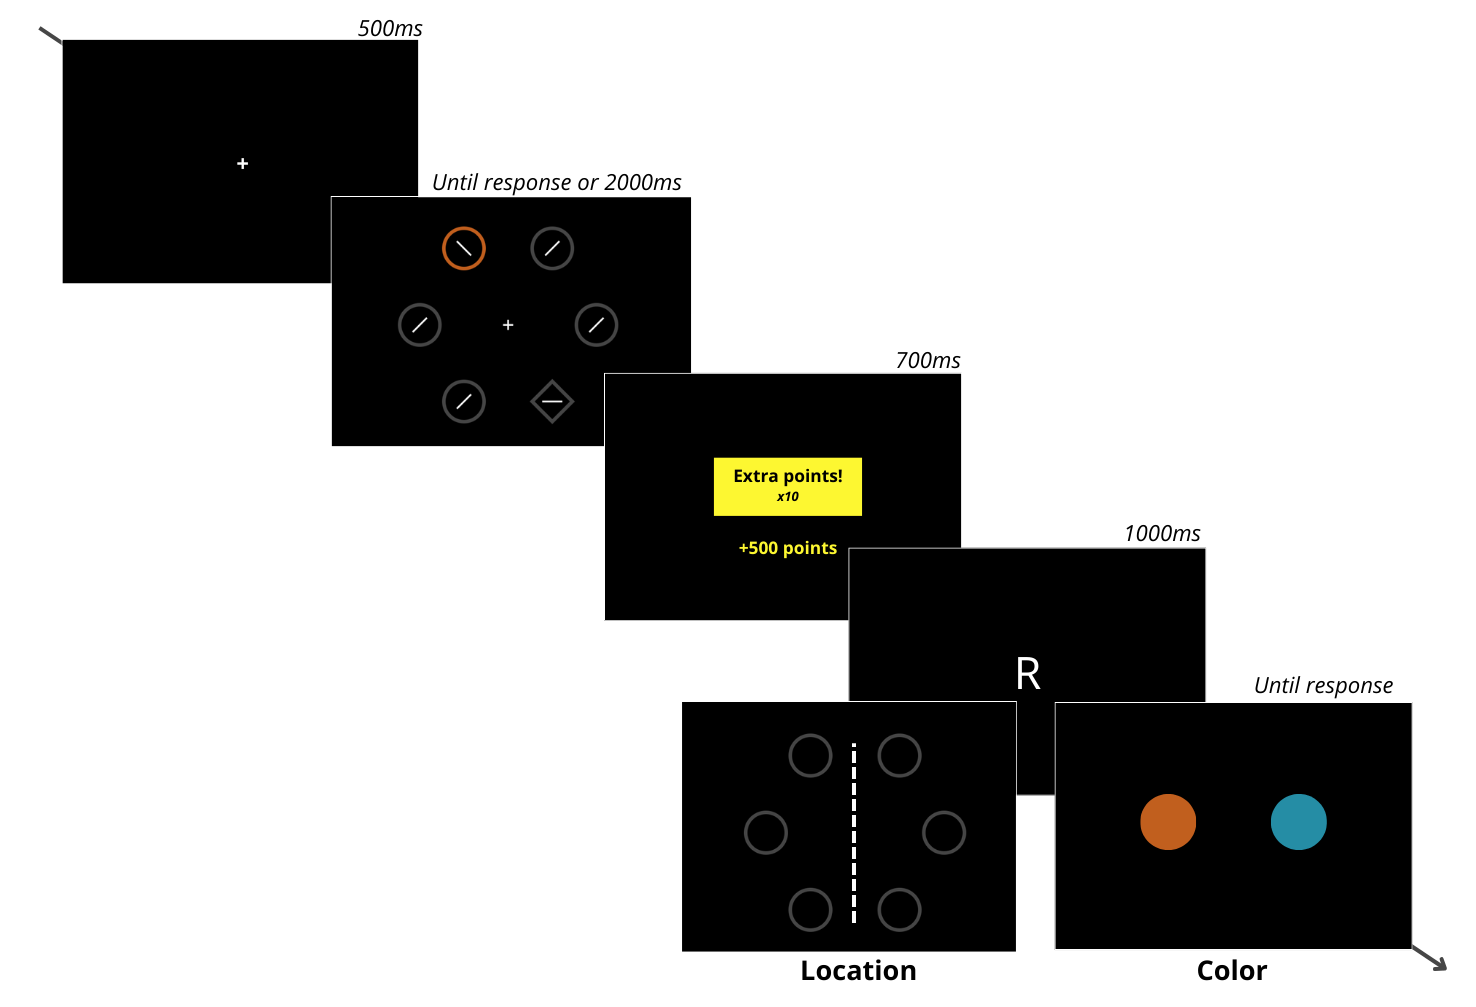
\includegraphics[keepaspectratio]{pre_registation/figure_3.png}}

{\noindent \emph{Note.} Example of the sequence of events in the
experimental task. Participants could earn points based on performance,
and when a high-value singleton appeared in the display, points were
multiplied by 10 (a bonus trial). In some trials, participants were
presented with the letter `R', which signaled that participants had to
report the color or the location (as a function of the assigned group)
of the distractor in the preceding trial. Feedback was provided in
Spanish.}

\end{figure}

Participants were randomly assigned to one of two groups, and each group
was required to perform a brief secondary task that occurred
pseudorandomly at the end of selected trials. One group reported the
color of the singleton distractor presented in the previous trial, while
the other group reported its location, indicating whether it appeared on
the left or right side of the display (Figure 1). Participants were
informed that the letter ``R'' would occasionally appear on the display
after the reward feedback, indicating that they had to report either the
color or the location of the distractor, depending on their assigned
group, using the \textless c\textgreater{} and \textless m\textgreater{}
keys to indicate left or right. To integrate the reporting task with the
visual search task, correct responses in the reporting task were worth
2000 points, while incorrect responses resulted in the loss of the same
number of points. However, feedback on performance on these trials was
provided only at the end of each block. Participants encountered either
two or four report trials per block, with at least one in the first half
and one in the second half of the block.

At the end of the experiment, participants completed an awareness test
to assess their knowledge of the color-reward contingencies using a
Visual Analog Scale (VAS; \citeproc{ref-Reips2008}{Reips \& Funke,
2008}). First, they rated the extent to which they believed that the
color of the distractor influenced the likelihood of ``bonus trials''
(\emph{contingency belief}), on a scale from 0 (``I don't believe color
makes any difference'') to 100 (``I believe color completely determines
the likelihood of bonus trials''). They then estimated the relative
proportion of bonus trials associated with each color (\emph{contingency
awareness}). To do this, they were presented with another VAS showing
the high- and low-rated distractors with endpoints indicating the
percentage of bonus trials estimated to be associated with each color.
After providing these ratings, participants indicated their confidence
in each answer using a confidence VAS ranging from 0 (``no confidence'')
to 100 (``very confident'').

\begin{figure*}[h]

{\caption{{Summary of results}{\label{fig-2}}}}

\pandocbounded{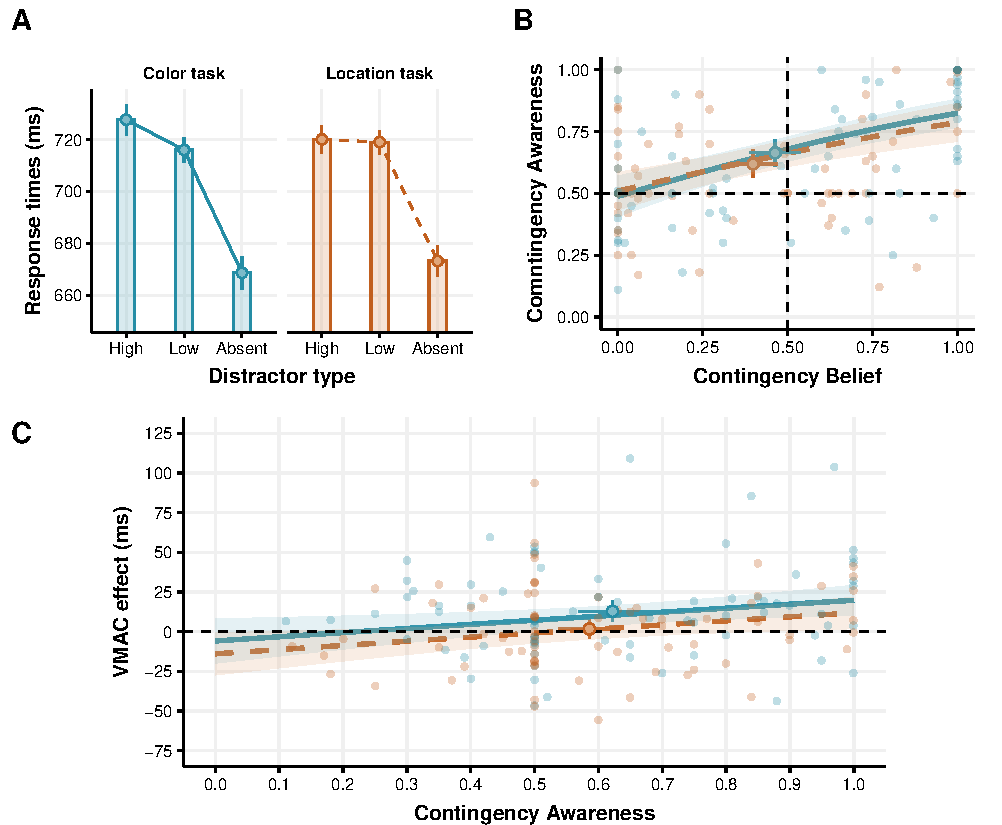
\includegraphics[keepaspectratio]{Output/plots/fig2.pdf}}

{\noindent \emph{Note.} \textbf{A}) Mean RTs in the visual search task.
Bars and dots show condition means; error bars indicate within-subject
95\% CIs (\citeproc{ref-morey2008}{Morey, 2008}). \textbf{B}) Beta
regression predictions for awareness results. Transparent dots are
individual responses; lines and shaded areas show model predictions and
95\% CIs. \textbf{C}) RT analysis with contingency awareness as
covariate. Transparent dots show individual VMAC scores; lines and
shaded areas depict model predictions by task and awareness level.
Solid, large dots and error bars show group means and 95\% CIs. Note
that only the group attending to color showed a positive VMAC effect
(blue dot), but the effect was independent of contingency awareness.}

\end{figure*}

\section{Results}\label{results}

All the analyses reported in this section follow our preregistered
analysis plan (\url{https://osf.io/f3bm8}). We excluded incorrect
responses (5.53\%), outliers (RTs \textless{} 150 or \textgreater{} 1800
ms; 0.57\%), and all trials from the first block of the visual search
task.

\subsection{Report task}\label{report-task}

We fitted a generalized linear mixed model (GLMM) with binomial
likelihood to analyze accuracy on the report task, including a group
predictor. Accuracy was high
(\(M_{\text{Accuracy}} = 0.946, \;95\%\,\text{CI}[0.933, 0.959]\)) and
did not differ significantly between groups (\emph{p} = 0.749),
suggesting that participants performed well on the secondary task.

\subsection{Visual search task}\label{visual-search-task}

We analyzed log-transformed RTs using linear mixed models that included
two predictors of theoretical interest: value-modulated attentional
capture (VMAC: high- vs.~low-value distractor) and attentional capture
(AC: low-value vs.~absent distractor), along with a Group predictor
(color vs.~location report task). As preregistered and following our
hypothesis, all contrasts were two-tailed except for the VMAC × Group
interaction, for which we used a one-tailed test in the direction of a
larger VMAC effect in the color group.

RT analyses showed significant effects of both AC and VMAC
(\(\beta_{\mathrm{VMAC}} = 0.008, \; t_{151} = 2.57, \; p = 0.011\);
\(\beta_{\mathrm{AC}} = 0.062, \; t_{151} = 17.26, \; p < 0.001\)),
indicating that participants were slower in the presence of a high-value
distractor
(\(M_{\mathrm{High}} = 734.2,\;95\%\,\mathrm{CI}[719.7, 748.9]\))
compared to a low-value distractor
(\(M_{\mathrm{Low}} = 728.4,\;95\%\,\mathrm{CI}[713.8, 743.3]\)), and
faster when no distractor was present
(\(M_{\mathrm{Absent}} = 684.2,\;95\%\,\mathrm{CI}[671.1, 697.6]\)).
Critically, the Group predictor interacted significantly only with VMAC
(\(\beta_{\mathrm{VMAC x Group}} = 0.006, \; t_{151} = 1.98, \; p = 0.025\);
Fig. 2A), such that a significant VMAC effect was observed in the color
group (\(M_{\mathrm{VMAC}} = 10.4,\;95\%\,\mathrm{CI}[4.0, 16.8]\)) but
not in the location group
(\(M_{\mathrm{VMAC}} = 1.2,\;95\%\,\mathrm{CI}[-5.3, 7.6]\))\footnote{As
  preregistered, we estimated the split-half reliability of the VMAC
  effect using the approach described by Garre-Frutos et al.
  (\citeproc{ref-garre-frutos2024}{2024}). Reliability was low
  (\(r_{\text{sb}} = 0.28, \;95\%\,\text{CI}[0.09, 0.44]\)), suggesting
  that the observed between-group difference may be attenuated
  (\citeproc{ref-karvelis}{Karvelis \& Diaconescu, 2025};
  \citeproc{ref-wiernik2020}{Wiernik \& Dahlke, 2020}; but see
  \citeproc{ref-parsons2018}{Parsons, 2018}).}. No other effects reached
significance (\emph{ps} \textgreater{} 0.133).

We also analyzed accuracy with a GLMM and a binomial likelihood.
Overall, accuracy was high
(\(M_{\text{Accuracy}} = 0.954, \;95\%\,\text{CI}[0.948, 0.959]\)) and
none of the predictors reached significance (\emph{ps} \textgreater{}
0.365).

\subsection{Awareness}\label{awareness}

Following our preregistered plan, we analyzed awareness measures using
beta regression (\citeproc{ref-smithson2006}{Smithson \& Verkuilen,
2006}). Neither measure differed significantly between groups (\emph{ps}
\textgreater{} 0.224). However, the two awareness measures were
significantly correlated (\(\beta = 0.551, \; z = 6.632, \; p < 0.001\);
Fig. 2B) with no significant group differences in this correlation
(\emph{p} = 0.444). While contingency awareness was positively
associated with confidence
(\(\beta = 0.579, \; z = 7.197, \; p < 0.001\); no group difference,
\emph{p} = 0.409), contingency belief was not (\emph{ps} \textgreater{}
0.231)\footnote{Note that this result only suggests that the
  relationship between contingency belief and confidence is less clear
  than contingency awareness, as participants with high contingency
  belief also report high contingency awareness.}.

As preregistered, we repeated the RT analysis restricted to high- and
low-value distractor trials, including contingency awareness and its
interaction with VMAC as covariates. This analysis revealed a
significant VMAC × awareness interaction
(\(\beta_{\mathrm{VMAC x Awareness}} = 0.008, \; t_{151} = 2.58, \; p = 0.011\)),
indicating a positive association (Figure 2C). However, the VMAC × Group
interaction remained significant
(\(\beta_{\mathrm{VMAC x Group}} = 0.006, \; t_{151} = 1.79, \; p = 0.038\)),
indicating that the interaction with selective attention cannot be
explained by individual differences in awareness alone.

\section{Discussion}\label{discussion}

In this preregistered study, we investigated the role of selective
attention in the learning process underlying VMAC. We manipulated
between groups whether participants reported the color or the location
of a distractor in a concurrent task, forcing selective attention to a
specific dimension of the distractor. Our results indicate that only
participants tasked with reporting color showed a significant VMAC
effect. Critically, the groups did not differ on any measure of
awareness, and the modulation of VMAC by task demands remained
significant even after controlling for individual differences in
awareness. However, individual differences in contingency awareness were
positively associated with VMAC, suggesting that both contingency
awareness and selective attention independently modulated the VMAC
effect.

The role of awareness in VMAC is controversial. Some studies suggest
that stimulus-reward associations can be learned without contingency
awareness (\citeproc{ref-anderson2015}{Anderson, 2015};
\citeproc{ref-anderson2013}{Anderson \& Yantis, 2013};
\citeproc{ref-gruxe9goire2019}{Grégoire \& Anderson, 2019};
\citeproc{ref-theeuwes2012}{Theeuwes \& Belopolsky, 2012}), while other
studies have found the opposite (\citeproc{ref-failing2017}{Failing \&
Theeuwes, 2017}; \citeproc{ref-garre-frutos2025a}{Garre-Frutos,
Lupiáñez, et al., 2025}; \citeproc{ref-lepelley2017}{Le Pelley et al.,
2017}; \citeproc{ref-meyer2020}{Meyer et al., 2020}). Consistent with
the latter, contingency instruction appears to be one of the strongest
moderators of the VMAC effect across studies
(\citeproc{ref-garre-frutos2025a}{Garre-Frutos, Lupiáñez, et al.,
2025}), mirroring findings from the human Pavlovian learning literature
(\citeproc{ref-lovibond2011}{Lovibond et al., 2011};
\citeproc{ref-mertens2016}{Mertens et al., 2016};
\citeproc{ref-mertens2020}{Mertens \& Engelhard, 2020};
\citeproc{ref-weidemann2016}{Weidemann et al., 2016}). Unlike other
learned attentional biases, such as visual statistical learning
(\citeproc{ref-wang2018}{Wang \& Theeuwes, 2018}), where either
bottom-up or top-down attention suffice for learning the statistical
contingencies (\citeproc{ref-duncan2024}{Duncan et al., 2024};
\citeproc{ref-duncan2020}{Duncan \& Theeuwes, 2020}), our results
suggest that VMAC specifically requires top-down attention to the
reward-associated feature, which can be induced by various factors,
including task relevance (\citeproc{ref-anderson2011}{Anderson et al.,
2011}), instructions, or knowledge of stimulus-reward contingencies
(\citeproc{ref-failing2017}{Failing \& Theeuwes, 2017};
\citeproc{ref-garre-frutos2025a}{Garre-Frutos, Lupiáñez, et al., 2025};
\citeproc{ref-lepelley2017}{Le Pelley et al., 2017};
\citeproc{ref-meyer2020}{Meyer et al., 2020}). According to classical
theories of automaticity, such as instance theory
(\citeproc{ref-jamieson2012}{Jamieson et al., 2012},
\citeproc{ref-jamieson2022}{2022}; \citeproc{ref-logan1988a}{Logan,
1988}, \citeproc{ref-logan2002}{2002}), the simplest explanation is that
selective attention determines what is learned
(\citeproc{ref-logan1996}{Logan et al., 1996},
\citeproc{ref-logan1999}{1999}; \citeproc{ref-logan1994}{Logan \&
Etherton, 1994}). According to this account, all previous moderators of
VMAC could operate by directing selective attention to the
reward-predictive feature, facilitating learning independent of
awareness (see also \citeproc{ref-jimuxe9nez1999}{Jiménez \& Méndez,
1999}). This idea might explain why null findings regarding VMAC and
awareness are particularly common in paradigms where the
reward-predictive feature is task-relevant during training. Consistent
with this interpretation, we observed that selective attention to
different distractor features in dual-task conditions was sufficient to
produce VMAC, suggesting that selective attention may be a necessary
(and sufficient) condition for learning.

We also found that VMAC significantly correlated with contingency
awareness, independent of the selective attention manipulation. Based on
the previous account, learning should depend not only on selective
attention to the reward-predictive feature, but also on reward feedback.
Thus, contingency awareness could reflect joint attention to both
elements, reflecting the same mechanism triggered by our manipulation.
However, the effect of awareness could also imply that propositional
knowledge triggers Pavlovian learning through a different mechanism
(\citeproc{ref-dayan2014}{Dayan \& Berridge, 2014};
\citeproc{ref-mitchell2009}{Mitchell et al., 2009};
\citeproc{ref-pauli2019}{Pauli et al., 2019}), or even that knowledge of
feature-reward associations might artificially amplify VMAC effect sizes
for reasons unrelated to Pavlovian learning, such as strategic attention
to high-value distractors to maximize information
(\citeproc{ref-doyle2025}{Doyle et al., 2025};
\citeproc{ref-gottlieb2014}{Gottlieb et al., 2014};
\citeproc{ref-mahlberg}{Mahlberg et al., 2025}) or the introduction of a
subtle speed-accuracy trade-off
(\citeproc{ref-garre-frutos2025b}{Garre-Frutos, Ariza, et al., 2025}).

In summary, our study shows that the relationship between attention and
VMAC can be mediated by selective attention to the reward-predictive
feature, even when it is irrelevant to the search task. This finding
underscores that VMAC requires selective attention to encode and
represent the contingency between features and rewards.

\section{References}\label{references}

\phantomsection\label{refs}
\begin{CSLReferences}{1}{0}
\bibitem[\citeproctext]{ref-anderson2015}
Anderson, B. A. (2015). Value-driven attentional priority is context
specific. \emph{Psychonomic Bulletin \& Review}, \emph{22}(3), 750--756.
\url{https://doi.org/10.3758/s13423-014-0724-0}

\bibitem[\citeproctext]{ref-anderson2021}
Anderson, B. A., Kim, H., Kim, A. J., Liao, M.-R., Mrkonja, L., Clement,
A., \& Grégoire, L. (2021). The past, present, and future of selection
history. \emph{Neuroscience \& Biobehavioral Reviews}, \emph{130},
326--350. \url{https://doi.org/10.1016/j.neubiorev.2021.09.004}

\bibitem[\citeproctext]{ref-anderson2011}
Anderson, B. A., Laurent, P. A., \& Yantis, S. (2011). Value-driven
attentional capture. \emph{Proceedings of the National Academy of
Sciences}, \emph{108}(25), 10367--10371.
\url{https://doi.org/10.1073/pnas.1104047108}

\bibitem[\citeproctext]{ref-anderson2013}
Anderson, B. A., \& Yantis, S. (2013). Persistence of value-driven
attentional capture. \emph{Journal of Experimental Psychology. Human
Perception and Performance}, \emph{39}(1), 6--9.
\url{https://doi.org/10.1037/a0030860}

\bibitem[\citeproctext]{ref-dayan2014}
Dayan, P., \& Berridge, K. C. (2014). Model-based and model-free
Pavlovian reward learning: Revaluation, revision, and revelation.
\emph{Cognitive, Affective, \& Behavioral Neuroscience}, \emph{14}(2),
473--492. \url{https://doi.org/10.3758/s13415-014-0277-8}

\bibitem[\citeproctext]{ref-doyle2025}
Doyle, A., Volkova, K., Crotty, N., Massa, N., \& Grubb, M. A. (2025).
Information-driven attentional capture. \emph{Attention, Perception, \&
Psychophysics}, \emph{87}(3), 721--727.
\url{https://doi.org/10.3758/s13414-024-03008-z}

\bibitem[\citeproctext]{ref-duncan2024}
Duncan, D., Moorselaar, D. van, \& Theeuwes, J. (2024). Visual
statistical learning requires attention. \emph{Psychonomic Bulletin \&
Review}. \url{https://doi.org/10.3758/s13423-024-02605-1}

\bibitem[\citeproctext]{ref-duncan2020}
Duncan, D., \& Theeuwes, J. (2020). Statistical learning in the absence
of explicit top-down attention. \emph{Cortex}, \emph{131}, 54--65.
\url{https://doi.org/10.1016/j.cortex.2020.07.006}

\bibitem[\citeproctext]{ref-failing2017}
Failing, M., \& Theeuwes, J. (2017). Don{'}t let it distract you: how
information about the availability of reward affects attentional
selection. \emph{Attention, Perception, \& Psychophysics}, \emph{79}(8),
2275--2298. \url{https://doi.org/10.3758/s13414-017-1376-8}

\bibitem[\citeproctext]{ref-failing2018}
Failing, M., \& Theeuwes, J. (2018). Selection history: How reward
modulates selectivity of visual attention. \emph{Psychonomic Bulletin \&
Review}, \emph{25}(2), 514--538.
\url{https://doi.org/10.3758/s13423-017-1380-y}

\bibitem[\citeproctext]{ref-gao2020}
Gao, Y., \& Theeuwes, J. (2020). Learning to suppress a distractor is
not affected by working memory load. \emph{Psychonomic Bulletin \&
Review}, \emph{27}(1), 96--104.
\url{https://doi.org/10.3758/s13423-019-01679-6}

\bibitem[\citeproctext]{ref-garre-frutos2025b}
Garre-Frutos, F., Ariza, A., \& González, F. (2025). The effect of
reward and punishment on the extinction of attentional capture elicited
by value-related stimuli. \emph{Psychological Research}, \emph{89}(3),
89. \url{https://doi.org/10.1007/s00426-025-02115-2}

\bibitem[\citeproctext]{ref-garre-frutos2025a}
Garre-Frutos, F., Lupiáñez, J., \& Vadillo, M. A. (2025).
\emph{Value-modulated attentional capture depends on awareness}.
PsyArXiv. \url{https://doi.org/10.31234/osf.io/hpexf}

\bibitem[\citeproctext]{ref-garre-frutos2024}
Garre-Frutos, F., Vadillo, M. A., González, F., \& Lupiáñez, J. (2024).
On the reliability of value-modulated attentional capture: An online
replication and multiverse analysis. \emph{Behavior Research Methods}.
\url{https://doi.org/10.3758/s13428-023-02329-5}

\bibitem[\citeproctext]{ref-gottlieb2014}
Gottlieb, J., Hayhoe, M., Hikosaka, O., \& Rangel, A. (2014). Attention,
Reward, and Information Seeking. \emph{Journal of Neuroscience},
\emph{34}(46), 15497--15504.
\url{https://doi.org/10.1523/JNEUROSCI.3270-14.2014}

\bibitem[\citeproctext]{ref-gruxe9goire2019}
Grégoire, L., \& Anderson, B. A. (2019). Semantic generalization of
value-based attentional priority. \emph{Learning \& Memory},
\emph{26}(12), 460--464. \url{https://doi.org/10.1101/lm.050336.119}

\bibitem[\citeproctext]{ref-jamieson2012}
Jamieson, R. K., Crump, M. J. C., \& Hannah, S. D. (2012). An instance
theory of associative learning. \emph{Learning \& Behavior},
\emph{40}(1), 61--82. \url{https://doi.org/10.3758/s13420-011-0046-2}

\bibitem[\citeproctext]{ref-jamieson2022}
Jamieson, R. K., Johns, B. T., Vokey, J. R., \& Jones, M. N. (2022).
Instance theory as a domain-general framework for cognitive psychology.
\emph{Nature Reviews Psychology}, \emph{1}(3), 174--183.
\url{https://doi.org/10.1038/s44159-022-00025-3}

\bibitem[\citeproctext]{ref-jiang2001}
Jiang, Y., \& Chun, M. M. (2001). Selective attention modulates implicit
learning. \emph{The Quarterly Journal of Experimental Psychology. A,
Human Experimental Psychology}, \emph{54}(4), 1105--1124.
\url{https://doi.org/10.1080/713756001}

\bibitem[\citeproctext]{ref-jimuxe9nez1999}
Jiménez, L., \& Méndez, C. (1999). Which attention is needed for
implicit sequence learning? \emph{Journal of Experimental Psychology:
Learning, Memory, and Cognition}, \emph{25}(1), 236--259.
\url{https://doi.org/10.1037/0278-7393.25.1.236}

\bibitem[\citeproctext]{ref-karvelis}
Karvelis, P., \& Diaconescu, A. (2025). \emph{Clarifying the reliability
paradox: Poor test-retest reliability attenuates group differences}.
\url{https://doi.org/10.31234/osf.io/z4yqe}

\bibitem[\citeproctext]{ref-lepelley2016}
Le Pelley, M. E., Mitchell, C. J., Beesley, T., George, D. N., \& Wills,
A. J. (2016). Attention and associative learning in humans: An
integrative review. \emph{Psychological Bulletin}, \emph{142}(10),
11111140. \url{https://doi.org/10.1037/bul0000064}

\bibitem[\citeproctext]{ref-lepelley2015}
Le Pelley, M. E., Pearson, D., Griffiths, O., \& Beesley, T. (2015).
When Goals Conflict With Values: Counterproductive Attentional and
Oculomotor Capture by Reward-Related Stimuli. \emph{Journal of
Experimental Psychology: General}, \emph{144}, 158--171.
https://doi.org/\url{http://dx.doi.org/10.1037/xge0000037}

\bibitem[\citeproctext]{ref-lepelley2017}
Le Pelley, M. E., Seabrooke, T., Kennedy, B. L., Pearson, D., \& Most,
S. B. (2017). Miss it and miss out: Counterproductive nonspatial
attentional capture by task-irrelevant, value-related stimuli.
\emph{Attention, Perception, \& Psychophysics}, \emph{79}(6),
1628--1642. \url{https://doi.org/10.3758/s13414-017-1346-1}

\bibitem[\citeproctext]{ref-logan1988a}
Logan, G. D. (1988). Toward an instance theory of automatization.
\emph{Psychological Review}, \emph{95}(4), 492--527.
\url{https://doi.org/10.1037/0033-295X.95.4.492}

\bibitem[\citeproctext]{ref-logan2002}
Logan, G. D. (2002). An instance theory of attention and memory.
\emph{Psychological Review}, \emph{109}(2), 376--400.
\url{https://doi.org/10.1037/0033-295X.109.2.376}

\bibitem[\citeproctext]{ref-logan1994}
Logan, G. D., \& Etherton, J. L. (1994). {"}What is learned during
automatization? The role of attention in constructing an instance{"}:
Correction to logan and etherton. \emph{Journal of Experimental
Psychology: Learning, Memory, and Cognition}, \emph{20}(6), 1390--1390.
\url{https://doi.org/10.1037/h0090354}

\bibitem[\citeproctext]{ref-logan1996}
Logan, G. D., Taylor, S. E., \& Etherton, J. L. (1996). Attention in the
acquisition and expression of automaticity. \emph{Journal of
Experimental Psychology: Learning, Memory, and Cognition}, \emph{22}(3),
620--638. \url{https://doi.org/10.1037/0278-7393.22.3.620}

\bibitem[\citeproctext]{ref-logan1999}
Logan, G. D., Taylor, S. E., \& Etherton, J. L. (1999). Attention and
automaticity: Toward a theoretical integration. \emph{Psychological
Research}, \emph{62}(2), 165--181.
\url{https://doi.org/10.1007/s004260050049}

\bibitem[\citeproctext]{ref-lovibond2011}
Lovibond, P. F., Liu, J. C. J., Weidemann, G., \& Mitchell, C. J.
(2011). Awareness is necessary for differential trace and delay eyeblink
conditioning in humans. \emph{Biological Psychology}, \emph{87}(3),
393--400. \url{https://doi.org/10.1016/j.biopsycho.2011.05.002}

\bibitem[\citeproctext]{ref-lovibond2002}
Lovibond, P. F., \& Shanks, D. R. (2002). The role of awareness in
pavlovian conditioning: Empirical evidence and theoretical implications.
\emph{Journal of Experimental Psychology: Animal Behavior Processes},
\emph{28}(1), 3--26. \url{https://doi.org/10.1037/0097-7403.28.1.3}

\bibitem[\citeproctext]{ref-mahlberg}
Mahlberg, J., Pearson, D., Le Pelley, M. E., \& Watson, P. (2025).
Prospective distractor information reduces reward-related attentional
capture. \emph{Journal of Cognition}, \emph{7}(1), 50.
\url{https://doi.org/10.5334/joc.375}

\bibitem[\citeproctext]{ref-mertens2020}
Mertens, G., \& Engelhard, I. M. (2020). A systematic review and
meta-analysis of the evidence for unaware fear conditioning.
\emph{Neuroscience \& Biobehavioral Reviews}, \emph{108}, 254--268.
\url{https://doi.org/10.1016/j.neubiorev.2019.11.012}

\bibitem[\citeproctext]{ref-mertens2016}
Mertens, G., Raes, A. K., \& De Houwer, J. (2016). Can prepared fear
conditioning result from verbal instructions? \emph{Learning and
Motivation}, \emph{53}, 7--23.
\url{https://doi.org/10.1016/j.lmot.2015.11.001}

\bibitem[\citeproctext]{ref-meyer2020}
Meyer, K. N., Sheridan, M. A., \& Hopfinger, J. B. (2020). Reward
history impacts attentional orienting and inhibitory control on
untrained tasks. \emph{Attention, Perception, \& Psychophysics},
\emph{82}(8), 3842--3862.
\url{https://doi.org/10.3758/s13414-020-02130-y}

\bibitem[\citeproctext]{ref-mitchell2009}
Mitchell, C. J., Houwer, J. D., \& Lovibond, P. F. (2009). The
propositional nature of human associative learning. \emph{Behavioral and
Brain Sciences}, \emph{32}(2), 183--198.
\url{https://doi.org/10.1017/S0140525X09000855}

\bibitem[\citeproctext]{ref-morey2008}
Morey, R. D. (2008). Confidence intervals from normalized data: A
correction to cousineau (2005). \emph{Tutorials in Quantitative Methods
for Psychology}, \emph{4}(2), 61--64.

\bibitem[\citeproctext]{ref-parsons2018}
Parsons, S. (2018). \emph{Visualising two approaches to explore
reliability-power relationships}. PsyArXiv.
\url{https://doi.org/10.31234/osf.io/qh5mf}

\bibitem[\citeproctext]{ref-pauli2019}
Pauli, W. M., Gentile, G., Collette, S., Tyszka, J. M., \& O'Doherty, J.
P. (2019). Evidence for model-based encoding of Pavlovian contingencies
in the human brain. \emph{Nature Communications}, \emph{10}(1), 1099.
\url{https://doi.org/10.1038/s41467-019-08922-7}

\bibitem[\citeproctext]{ref-pearson2016}
Pearson, D., Osborn, R., Whitford, T. J., Failing, M., Theeuwes, J., \&
Le Pelley, M. E. (2016). Value-modulated oculomotor capture by
task-irrelevant stimuli is a consequence of early competition on the
saccade map. \emph{Attention, Perception, \& Psychophysics},
\emph{78}(7), 2226--2240.
\url{https://doi.org/10.3758/s13414-016-1135-2}

\bibitem[\citeproctext]{ref-Reips2008}
Reips, U.-D., \& Funke, F. (2008). Interval-level measurement with
visual analogue scales in internet-based research: VAS generator.
\emph{Behavior Research Methods}, \emph{40}(3), 699--704.
\url{https://doi.org/10.3758/BRM.40.3.699}

\bibitem[\citeproctext]{ref-smithson2006}
Smithson, M., \& Verkuilen, J. (2006). A better lemon squeezer?
Maximum-likelihood regression with beta-distributed dependent variables.
\emph{Psychological Methods}, \emph{11}(1), 54--71.
\url{https://doi.org/10.1037/1082-989X.11.1.54}

\bibitem[\citeproctext]{ref-theeuwes1992}
Theeuwes, J. (1992). Perceptual selectivity for color and form.
\emph{Perception \& Psychophysics}, \emph{51}(6), 599--606.
\url{https://doi.org/10.3758/BF03211656}

\bibitem[\citeproctext]{ref-theeuwes1994}
Theeuwes, J. (1994). Stimulus-driven capture and attentional set:
Selective search for color and visual abrupt onsets. \emph{Journal of
Experimental Psychology: Human Perception and Performance},
\emph{20}(4), 799--806. \url{https://doi.org/10.1037/0096-1523.20.4.799}

\bibitem[\citeproctext]{ref-theeuwes2012}
Theeuwes, J., \& Belopolsky, A. V. (2012). Reward grabs the eye:
Oculomotor capture by rewarding stimuli. \emph{Vision Research},
\emph{74}, 80--85. \url{https://doi.org/10.1016/j.visres.2012.07.024}

\bibitem[\citeproctext]{ref-vadillo2024}
Vadillo, M. A., Aniento, P., Hernández-Gutiérrez, D., Saini, L., \&
Aivar, M. P. (2024). Measuring learning and attention to irrelevant
distractors in contextual cueing. \emph{Journal of Experimental
Psychology: Human Perception and Performance}, \emph{50}(9), 952--970.
\url{https://doi.org/10.1037/xhp0001230}

\bibitem[\citeproctext]{ref-vadillo2020}
Vadillo, M. A., Giménez-Fernández, T., Aivar, M. P., \& Cubillas, C. P.
(2020). Ignored visual context does not induce latent learning.
\emph{Psychonomic Bulletin \& Review}, \emph{27}(3), 512--519.
\url{https://doi.org/10.3758/s13423-020-01722-x}

\bibitem[\citeproctext]{ref-wang2018}
Wang, B., \& Theeuwes, J. (2018). Statistical regularities modulate
attentional capture. \emph{Journal of Experimental Psychology: Human
Perception and Performance}, \emph{44}(1), 13--17.
\url{https://doi.org/10.1037/xhp0000472}

\bibitem[\citeproctext]{ref-weidemann2016}
Weidemann, G., Satkunarajah, M., \& Lovibond, P. F. (2016). I Think,
Therefore Eyeblink: The Importance of Contingency Awareness in
Conditioning. \emph{Psychological Science}, \emph{27}(4), 467--475.
\url{https://doi.org/10.1177/0956797615625973}

\bibitem[\citeproctext]{ref-wiernik2020}
Wiernik, B. M., \& Dahlke, J. A. (2020). Obtaining unbiased results in
meta-analysis: The importance of correcting for statistical artifacts.
\emph{Advances in Methods and Practices in Psychological Science},
\emph{3}(1), 94--123. \url{https://doi.org/10.1177/2515245919885611}

\bibitem[\citeproctext]{ref-anderson2015}
Anderson, B. A. (2015). Value-driven attentional priority is context
specific. \emph{Psychonomic Bulletin \& Review}, \emph{22}(3), 750--756.
\url{https://doi.org/10.3758/s13423-014-0724-0}

\bibitem[\citeproctext]{ref-anderson2021}
Anderson, B. A., Kim, H., Kim, A. J., Liao, M.-R., Mrkonja, L., Clement,
A., \& Grégoire, L. (2021). The past, present, and future of selection
history. \emph{Neuroscience \& Biobehavioral Reviews}, \emph{130},
326--350. \url{https://doi.org/10.1016/j.neubiorev.2021.09.004}

\bibitem[\citeproctext]{ref-anderson2011}
Anderson, B. A., Laurent, P. A., \& Yantis, S. (2011). Value-driven
attentional capture. \emph{Proceedings of the National Academy of
Sciences}, \emph{108}(25), 10367--10371.
\url{https://doi.org/10.1073/pnas.1104047108}

\bibitem[\citeproctext]{ref-anderson2013}
Anderson, B. A., \& Yantis, S. (2013). Persistence of value-driven
attentional capture. \emph{Journal of Experimental Psychology. Human
Perception and Performance}, \emph{39}(1), 6--9.
\url{https://doi.org/10.1037/a0030860}

\bibitem[\citeproctext]{ref-dayan2014}
Dayan, P., \& Berridge, K. C. (2014). Model-based and model-free
Pavlovian reward learning: Revaluation, revision, and revelation.
\emph{Cognitive, Affective, \& Behavioral Neuroscience}, \emph{14}(2),
473--492. \url{https://doi.org/10.3758/s13415-014-0277-8}

\bibitem[\citeproctext]{ref-doyle2025}
Doyle, A., Volkova, K., Crotty, N., Massa, N., \& Grubb, M. A. (2025).
Information-driven attentional capture. \emph{Attention, Perception, \&
Psychophysics}, \emph{87}(3), 721--727.
\url{https://doi.org/10.3758/s13414-024-03008-z}

\bibitem[\citeproctext]{ref-duncan2024}
Duncan, D., Moorselaar, D. van, \& Theeuwes, J. (2024). Visual
statistical learning requires attention. \emph{Psychonomic Bulletin \&
Review}. \url{https://doi.org/10.3758/s13423-024-02605-1}

\bibitem[\citeproctext]{ref-duncan2020}
Duncan, D., \& Theeuwes, J. (2020). Statistical learning in the absence
of explicit top-down attention. \emph{Cortex}, \emph{131}, 54--65.
\url{https://doi.org/10.1016/j.cortex.2020.07.006}

\bibitem[\citeproctext]{ref-failing2017}
Failing, M., \& Theeuwes, J. (2017). Don{'}t let it distract you: how
information about the availability of reward affects attentional
selection. \emph{Attention, Perception, \& Psychophysics}, \emph{79}(8),
2275--2298. \url{https://doi.org/10.3758/s13414-017-1376-8}

\bibitem[\citeproctext]{ref-failing2018}
Failing, M., \& Theeuwes, J. (2018). Selection history: How reward
modulates selectivity of visual attention. \emph{Psychonomic Bulletin \&
Review}, \emph{25}(2), 514--538.
\url{https://doi.org/10.3758/s13423-017-1380-y}

\bibitem[\citeproctext]{ref-gao2020}
Gao, Y., \& Theeuwes, J. (2020). Learning to suppress a distractor is
not affected by working memory load. \emph{Psychonomic Bulletin \&
Review}, \emph{27}(1), 96--104.
\url{https://doi.org/10.3758/s13423-019-01679-6}

\bibitem[\citeproctext]{ref-garre-frutos2025b}
Garre-Frutos, F., Ariza, A., \& González, F. (2025). The effect of
reward and punishment on the extinction of attentional capture elicited
by value-related stimuli. \emph{Psychological Research}, \emph{89}(3),
89. \url{https://doi.org/10.1007/s00426-025-02115-2}

\bibitem[\citeproctext]{ref-garre-frutos2025a}
Garre-Frutos, F., Lupiáñez, J., \& Vadillo, M. A. (2025).
\emph{Value-modulated attentional capture depends on awareness}.
PsyArXiv. \url{https://doi.org/10.31234/osf.io/hpexf}

\bibitem[\citeproctext]{ref-garre-frutos2024}
Garre-Frutos, F., Vadillo, M. A., González, F., \& Lupiáñez, J. (2024).
On the reliability of value-modulated attentional capture: An online
replication and multiverse analysis. \emph{Behavior Research Methods}.
\url{https://doi.org/10.3758/s13428-023-02329-5}

\bibitem[\citeproctext]{ref-gottlieb2014}
Gottlieb, J., Hayhoe, M., Hikosaka, O., \& Rangel, A. (2014). Attention,
Reward, and Information Seeking. \emph{Journal of Neuroscience},
\emph{34}(46), 15497--15504.
\url{https://doi.org/10.1523/JNEUROSCI.3270-14.2014}

\bibitem[\citeproctext]{ref-gruxe9goire2019}
Grégoire, L., \& Anderson, B. A. (2019). Semantic generalization of
value-based attentional priority. \emph{Learning \& Memory},
\emph{26}(12), 460--464. \url{https://doi.org/10.1101/lm.050336.119}

\bibitem[\citeproctext]{ref-jamieson2012}
Jamieson, R. K., Crump, M. J. C., \& Hannah, S. D. (2012). An instance
theory of associative learning. \emph{Learning \& Behavior},
\emph{40}(1), 61--82. \url{https://doi.org/10.3758/s13420-011-0046-2}

\bibitem[\citeproctext]{ref-jamieson2022}
Jamieson, R. K., Johns, B. T., Vokey, J. R., \& Jones, M. N. (2022).
Instance theory as a domain-general framework for cognitive psychology.
\emph{Nature Reviews Psychology}, \emph{1}(3), 174--183.
\url{https://doi.org/10.1038/s44159-022-00025-3}

\bibitem[\citeproctext]{ref-jiang2001}
Jiang, Y., \& Chun, M. M. (2001). Selective attention modulates implicit
learning. \emph{The Quarterly Journal of Experimental Psychology. A,
Human Experimental Psychology}, \emph{54}(4), 1105--1124.
\url{https://doi.org/10.1080/713756001}

\bibitem[\citeproctext]{ref-jimuxe9nez1999}
Jiménez, L., \& Méndez, C. (1999). Which attention is needed for
implicit sequence learning? \emph{Journal of Experimental Psychology:
Learning, Memory, and Cognition}, \emph{25}(1), 236--259.
\url{https://doi.org/10.1037/0278-7393.25.1.236}

\bibitem[\citeproctext]{ref-karvelis}
Karvelis, P., \& Diaconescu, A. (2025). \emph{Clarifying the reliability
paradox: Poor test-retest reliability attenuates group differences}.
\url{https://doi.org/10.31234/osf.io/z4yqe}

\bibitem[\citeproctext]{ref-lepelley2016}
Le Pelley, M. E., Mitchell, C. J., Beesley, T., George, D. N., \& Wills,
A. J. (2016). Attention and associative learning in humans: An
integrative review. \emph{Psychological Bulletin}, \emph{142}(10),
11111140. \url{https://doi.org/10.1037/bul0000064}

\bibitem[\citeproctext]{ref-lepelley2015}
Le Pelley, M. E., Pearson, D., Griffiths, O., \& Beesley, T. (2015).
When Goals Conflict With Values: Counterproductive Attentional and
Oculomotor Capture by Reward-Related Stimuli. \emph{Journal of
Experimental Psychology: General}, \emph{144}, 158--171.
https://doi.org/\url{http://dx.doi.org/10.1037/xge0000037}

\bibitem[\citeproctext]{ref-lepelley2017}
Le Pelley, M. E., Seabrooke, T., Kennedy, B. L., Pearson, D., \& Most,
S. B. (2017). Miss it and miss out: Counterproductive nonspatial
attentional capture by task-irrelevant, value-related stimuli.
\emph{Attention, Perception, \& Psychophysics}, \emph{79}(6),
1628--1642. \url{https://doi.org/10.3758/s13414-017-1346-1}

\bibitem[\citeproctext]{ref-logan1988a}
Logan, G. D. (1988). Toward an instance theory of automatization.
\emph{Psychological Review}, \emph{95}(4), 492--527.
\url{https://doi.org/10.1037/0033-295X.95.4.492}

\bibitem[\citeproctext]{ref-logan2002}
Logan, G. D. (2002). An instance theory of attention and memory.
\emph{Psychological Review}, \emph{109}(2), 376--400.
\url{https://doi.org/10.1037/0033-295X.109.2.376}

\bibitem[\citeproctext]{ref-logan1994}
Logan, G. D., \& Etherton, J. L. (1994). {"}What is learned during
automatization? The role of attention in constructing an instance{"}:
Correction to logan and etherton. \emph{Journal of Experimental
Psychology: Learning, Memory, and Cognition}, \emph{20}(6), 1390--1390.
\url{https://doi.org/10.1037/h0090354}

\bibitem[\citeproctext]{ref-logan1996}
Logan, G. D., Taylor, S. E., \& Etherton, J. L. (1996). Attention in the
acquisition and expression of automaticity. \emph{Journal of
Experimental Psychology: Learning, Memory, and Cognition}, \emph{22}(3),
620--638. \url{https://doi.org/10.1037/0278-7393.22.3.620}

\bibitem[\citeproctext]{ref-logan1999}
Logan, G. D., Taylor, S. E., \& Etherton, J. L. (1999). Attention and
automaticity: Toward a theoretical integration. \emph{Psychological
Research}, \emph{62}(2), 165--181.
\url{https://doi.org/10.1007/s004260050049}

\bibitem[\citeproctext]{ref-lovibond2011}
Lovibond, P. F., Liu, J. C. J., Weidemann, G., \& Mitchell, C. J.
(2011). Awareness is necessary for differential trace and delay eyeblink
conditioning in humans. \emph{Biological Psychology}, \emph{87}(3),
393--400. \url{https://doi.org/10.1016/j.biopsycho.2011.05.002}

\bibitem[\citeproctext]{ref-lovibond2002}
Lovibond, P. F., \& Shanks, D. R. (2002). The role of awareness in
pavlovian conditioning: Empirical evidence and theoretical implications.
\emph{Journal of Experimental Psychology: Animal Behavior Processes},
\emph{28}(1), 3--26. \url{https://doi.org/10.1037/0097-7403.28.1.3}

\bibitem[\citeproctext]{ref-mahlberg}
Mahlberg, J., Pearson, D., Le Pelley, M. E., \& Watson, P. (2025).
Prospective distractor information reduces reward-related attentional
capture. \emph{Journal of Cognition}, \emph{7}(1), 50.
\url{https://doi.org/10.5334/joc.375}

\bibitem[\citeproctext]{ref-mertens2020}
Mertens, G., \& Engelhard, I. M. (2020). A systematic review and
meta-analysis of the evidence for unaware fear conditioning.
\emph{Neuroscience \& Biobehavioral Reviews}, \emph{108}, 254--268.
\url{https://doi.org/10.1016/j.neubiorev.2019.11.012}

\bibitem[\citeproctext]{ref-mertens2016}
Mertens, G., Raes, A. K., \& De Houwer, J. (2016). Can prepared fear
conditioning result from verbal instructions? \emph{Learning and
Motivation}, \emph{53}, 7--23.
\url{https://doi.org/10.1016/j.lmot.2015.11.001}

\bibitem[\citeproctext]{ref-meyer2020}
Meyer, K. N., Sheridan, M. A., \& Hopfinger, J. B. (2020). Reward
history impacts attentional orienting and inhibitory control on
untrained tasks. \emph{Attention, Perception, \& Psychophysics},
\emph{82}(8), 3842--3862.
\url{https://doi.org/10.3758/s13414-020-02130-y}

\bibitem[\citeproctext]{ref-mitchell2009}
Mitchell, C. J., Houwer, J. D., \& Lovibond, P. F. (2009). The
propositional nature of human associative learning. \emph{Behavioral and
Brain Sciences}, \emph{32}(2), 183--198.
\url{https://doi.org/10.1017/S0140525X09000855}

\bibitem[\citeproctext]{ref-morey2008}
Morey, R. D. (2008). Confidence intervals from normalized data: A
correction to cousineau (2005). \emph{Tutorials in Quantitative Methods
for Psychology}, \emph{4}(2), 61--64.

\bibitem[\citeproctext]{ref-parsons2018}
Parsons, S. (2018). \emph{Visualising two approaches to explore
reliability-power relationships}. PsyArXiv.
\url{https://doi.org/10.31234/osf.io/qh5mf}

\bibitem[\citeproctext]{ref-pauli2019}
Pauli, W. M., Gentile, G., Collette, S., Tyszka, J. M., \& O'Doherty, J.
P. (2019). Evidence for model-based encoding of Pavlovian contingencies
in the human brain. \emph{Nature Communications}, \emph{10}(1), 1099.
\url{https://doi.org/10.1038/s41467-019-08922-7}

\bibitem[\citeproctext]{ref-pearson2016}
Pearson, D., Osborn, R., Whitford, T. J., Failing, M., Theeuwes, J., \&
Le Pelley, M. E. (2016). Value-modulated oculomotor capture by
task-irrelevant stimuli is a consequence of early competition on the
saccade map. \emph{Attention, Perception, \& Psychophysics},
\emph{78}(7), 2226--2240.
\url{https://doi.org/10.3758/s13414-016-1135-2}

\bibitem[\citeproctext]{ref-Reips2008}
Reips, U.-D., \& Funke, F. (2008). Interval-level measurement with
visual analogue scales in internet-based research: VAS generator.
\emph{Behavior Research Methods}, \emph{40}(3), 699--704.
\url{https://doi.org/10.3758/BRM.40.3.699}

\bibitem[\citeproctext]{ref-smithson2006}
Smithson, M., \& Verkuilen, J. (2006). A better lemon squeezer?
Maximum-likelihood regression with beta-distributed dependent variables.
\emph{Psychological Methods}, \emph{11}(1), 54--71.
\url{https://doi.org/10.1037/1082-989X.11.1.54}

\bibitem[\citeproctext]{ref-theeuwes1992}
Theeuwes, J. (1992). Perceptual selectivity for color and form.
\emph{Perception \& Psychophysics}, \emph{51}(6), 599--606.
\url{https://doi.org/10.3758/BF03211656}

\bibitem[\citeproctext]{ref-theeuwes1994}
Theeuwes, J. (1994). Stimulus-driven capture and attentional set:
Selective search for color and visual abrupt onsets. \emph{Journal of
Experimental Psychology: Human Perception and Performance},
\emph{20}(4), 799--806. \url{https://doi.org/10.1037/0096-1523.20.4.799}

\bibitem[\citeproctext]{ref-theeuwes2012}
Theeuwes, J., \& Belopolsky, A. V. (2012). Reward grabs the eye:
Oculomotor capture by rewarding stimuli. \emph{Vision Research},
\emph{74}, 80--85. \url{https://doi.org/10.1016/j.visres.2012.07.024}

\bibitem[\citeproctext]{ref-vadillo2024}
Vadillo, M. A., Aniento, P., Hernández-Gutiérrez, D., Saini, L., \&
Aivar, M. P. (2024). Measuring learning and attention to irrelevant
distractors in contextual cueing. \emph{Journal of Experimental
Psychology: Human Perception and Performance}, \emph{50}(9), 952--970.
\url{https://doi.org/10.1037/xhp0001230}

\bibitem[\citeproctext]{ref-vadillo2020}
Vadillo, M. A., Giménez-Fernández, T., Aivar, M. P., \& Cubillas, C. P.
(2020). Ignored visual context does not induce latent learning.
\emph{Psychonomic Bulletin \& Review}, \emph{27}(3), 512--519.
\url{https://doi.org/10.3758/s13423-020-01722-x}

\bibitem[\citeproctext]{ref-wang2018}
Wang, B., \& Theeuwes, J. (2018). Statistical regularities modulate
attentional capture. \emph{Journal of Experimental Psychology: Human
Perception and Performance}, \emph{44}(1), 13--17.
\url{https://doi.org/10.1037/xhp0000472}

\bibitem[\citeproctext]{ref-weidemann2016}
Weidemann, G., Satkunarajah, M., \& Lovibond, P. F. (2016). I Think,
Therefore Eyeblink: The Importance of Contingency Awareness in
Conditioning. \emph{Psychological Science}, \emph{27}(4), 467--475.
\url{https://doi.org/10.1177/0956797615625973}

\bibitem[\citeproctext]{ref-wiernik2020}
Wiernik, B. M., \& Dahlke, J. A. (2020). Obtaining unbiased results in
meta-analysis: The importance of correcting for statistical artifacts.
\emph{Advances in Methods and Practices in Psychological Science},
\emph{3}(1), 94--123. \url{https://doi.org/10.1177/2515245919885611}

\end{CSLReferences}






\end{document}
